\documentclass[12pt]{article}

\usepackage[margin=1in]{geometry}
\usepackage[]{graphicx}

\title{Low-Power Machine Learning}
\author{Joe Redmon and Calvin Loncaric}
\date{June 12, 2014}

\begin{document}

\maketitle

\section{Introduction}

Low-power computing devices are becoming increasingly relevant. As computing
becomes more common, it will be more and more important to reduce power costs.
Low-power devices can be deployed in more areas where a steady supply of
electricity may be harder to come by. Lowering power requirements can increase
usability by increasing battery life. Battery-free devices that harvest energy
from ambient sources (such as radio waves) can be manufactured more cheaply
than battery-powered devices. As they have no battery, they are also more
environmentally friendly.

Previous work has established that gesture recognition on low-power devices is
possible \cite{allsee}. This means that low-power devices can augment or
replace high-power gesture recognition technologies. However, the set of
gestures available must be hard-coded in advance and carefully tuned for the
low-power environment. In this work we seek to remove this restriction by doing
simple machine learning on the device itself, enabling users to train new
gestures and removing the need for implementors to devise specialized
algorithms.

Machine learning has been successfully applied in almost every real-world
setting: control systems, computer vision, speech recognition, language
processing, signal processing, information retrieval, and many other domains.
Given its ubiquity, bringing machine learning to low-power devices could have
other applications as well. Control systems---such as those in thermostats---%
can learn patterns in their environment to better predict temperature changes
and adjust in advance. In the context of localization, machine learning could
enable devices to learn to differentiate various different locations by using
various sensors (as in SurroundSense \cite{surroundsense}). By pressing a
button a user could effectively train a new relevant location into the device.

Our work focuses on gesture recognition and has resulted in a small working
prototype based on the MSP430 line of low-power CPUs. By pressing buttons the
user can train a gesture into the prototype by performing it only twice.

\section{Background and Related Work}

Machine learning typically takes place in two phases. In the first phase
(``learning''), training data is used to construct a model. The model captures
with relatively little data the relationships in the training data and is used
in the second phase (``deployment'') along with input data to classify inputs
or predict outputs.

There has been previous work on producing models for low-power environments
\cite{low-power-models} but this work relies on a powerful external system to
produce the model in the first place. This makes it inappropriate for our
domain, as learning cannot be performed on the device itself.

Other groups have attempted to make learning low-power by producing dedicated
hardware \cite{ml-on-a-chip}. This work, while orders of magnitude more
power efficient than conventional hardware, still uses several
orders of magnitude more power than we would like. Their hardware requires
roughly 47300{$\mu$}W of power to run, while we expect to use under 50{$\mu$}W of
power. Dedicated hardware could become important if machine learning is
required in a low-power environment, but we would prefer an approach that runs
on general-purpose hardware so the device can be used for other things when
learning is not taking place.

A simpler learning algorithm that is still relatively high-accurracy is
required in this domain.

\section{Implementation}
Our implementation uses a two-phase procedure to learn to recognize gestures. First it learns the ground truth for the gesture and then it estimates the size of the space that should be classified as the gesture. Subsequent gestures are compared to this space to see if they match the trained gesture. The whole training and recognition procedure takes place on low power hardware that is suitable for RF powered devices.

\subsection{Hardware}
For prototyping our algorithm we used a MSP430 microcontroller on a LaunchPad development board and a MMA8452 accelerometer. The MSP430 consumes 500{$\mu$}W of power during active operation, but only 0.1{$\mu$}W when it is in low power mode. The MMA8452 uses 16{$\mu$}W of power when collecting samples. Sampling and processing both happen in a one off manner and are driven by user input so the system is usually in low power mode.

\subsection{Training}
When the user presses the input button, the device begins recording movement from the accelerometer. The first time the button is pressed, the sample is saved as the ground truth of the gesture. We sample for 2 seconds at 12.5 Hz, obtaining 25 readings. However, only the middle 15 (1.2 seconds) are used to eliminate noise at the beginning or end of the gesture.

The second time the button is pressed, the user performs the same action during the same time frame. We slide the ground truth gesture over the second buffer and find the window with the smallest difference:

\begin{equation}
\label{eq:norm}
\delta = \min_i \|V_{test}[i:i+15] - V_{truth} \|_1
\end{equation}

Using this $\delta$ we calculate our threshold $T = 1.5*\delta$

\subsection{Testing}
The full gesture model is specified by the ground truth vector $V_{test}$ and the threshold $T$. When the user presses the button again, we sample from the accelerometer and use equation \ref{eq:norm} to find the smallest overlap $\delta_{test}$. If $\delta_{test} < T$ than we classify the gesture as matching the trained gesture. If not, we reject it.

\begin{figure}[h]
\begin{center}
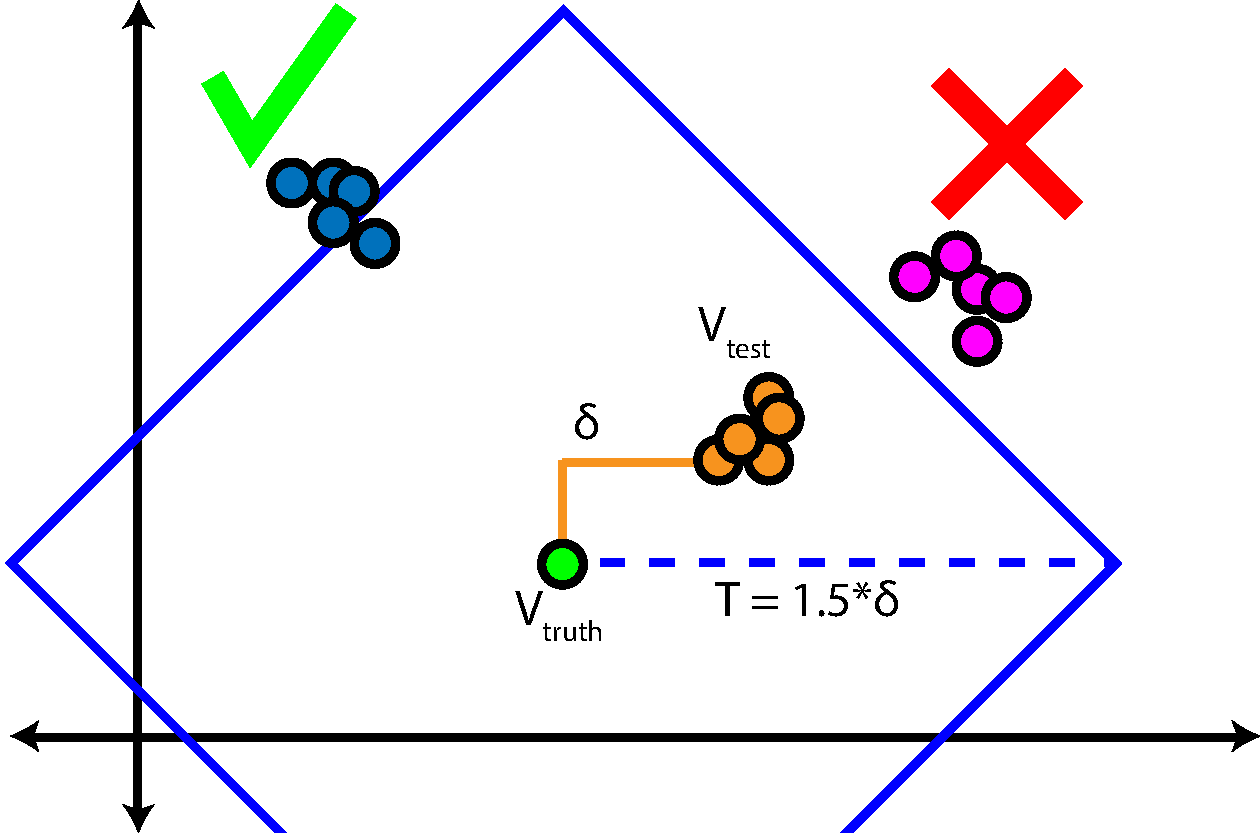
\includegraphics[width=.7\linewidth]{graph}
\end{center}
\caption{Our learning procedure. We learn the ground truth $V_{truth}$ and the threshold $T$. New examples are classified positive or negative based on their closest subvector.}
\label{graph}
\end{figure}


\section{Results and Discussion}

\section{Conclusion}

\bibliography{bibliography}
\bibliographystyle{plain}

\end{document}
